\documentclass{article}

\usepackage[utf8]{inputenc}
\usepackage[croatian]{babel}
\usepackage{graphicx}
\usepackage{caption}
\usepackage{subcaption}
\usepackage{amsmath}

\renewcommand{\figurename}{Slika}

\title{NENR - 7. domaća zadaća: Neuroračunarstvo i
evolucijsko računanje}
\author{Mate Gašparini}
\date{Zagreb, prosinac, 2019.}

\begin{document}

\maketitle

\section*{Zadatak 1.}
Razmotrite jedan neuron koji ima samo jedan ulaz. Njegov izlaz
tada će biti određen izrazom:
\begin{equation*}
    y = \frac{1}{1 + \frac{|x-w|}{|s|}}.
\end{equation*}
Pretpostavite da je u neuron pohranjena vrijednost $ w = 2 $.
Nacrtajte na istom grafu ovisnost $ y(x; w = 2) $ za tri
slučaja: za $ s = 1 $, za $ s = 0.25 $ te za $ s = 4 $ (svaku
različitom bojom ili stilom linije). Za raspon apscise uzmite
interval $ [-8, 10] $. Razumijete li sada kako $ s $ utječe
na izlaz neurona $ y $? Kako će izgledati izlaz neurona koji
ima dva ulaza i što se tada kontrolira parametrima $ s_1 $ i
$ s_2 $?

\section*{Rješenje:}
Na slici \ref{z1-1} prikazani su grafovi ovisnosti
$ y(x; w = 2) $ za različite vrijednosti parametra $ s $.

Što je veća vrijednost parametra $ s $, vrijednost izlaza
neurona $ y $ sporije opada udaljavanjem od točke $ x = w $.

U ovom primjeru neuron ima samo jedan ulaz te je
parametriziran parametrima $ w $ i $ s $. U slučaju neurona
koji ima dva ulaza, postojalo bi sveukupno 4 parametra:
$ w_1 $, $ w_2 $, $ s_1 $, $ s_2$. Parametri $ w_1 $ i
$ w_2 $ određivali bi točku maksimuma izlaza neurona $ y $,
dok bi parametri $ s_1 $ i $ s_2 $ određivali brzinu opadanja
vrijednosti $ y $ udaljavanjem vrijednosti $ x_1 $ od $ w_1 $
i $ x_2 $ od $ w_2 $.

\begin{figure}
    \centering
    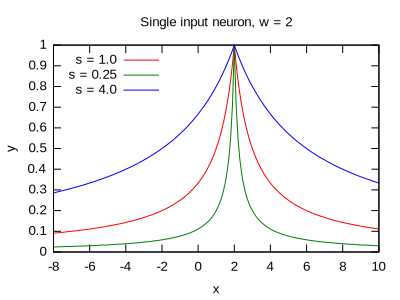
\includegraphics{img/task1-plot.pdf}
    \caption{Grafovi ovisnosti $ y(x; w = 2) $
    za različite vrijednosti parametra $ s $}
    \label{z1-1}
\end{figure}

\pagebreak

\section*{Zadatak 2.}
Iskoristite neki gotov program (ili napišite vlastiti
program, što god Vam je lakše) kako biste dobili 2D prikaz
podataka koje ste dobili za učenje
(\texttt{zad7}-\texttt{dataset.txt}). Pri tome uzorke
različitih razreda prikažite ili različitim simbolom (npr.
kvadratić, trokutić, kružić) ili različitom bojom. Ovu sliku
spremite kao dio Vaše dokumentacije. Ako ste koristili gotov
program, navedite naziv programa.\\
Proučite dobiveni prikaz. Postoji li kakav uzorak u tim
podatcima? Jesu li razredi međusobno linearno odvojivi?

\section*{Rješenje:}
Na slici \ref{z2-1} prikazan je skup podataka za učenje.
Uzorci su dvodimenzionalni, a ima ih sveukupno 64. Razvrstani
su u 3 različita razreda, kao što je različitim simbolima na
slici i prikazano.

Uzorci su raspoređeni u 8 ovalnih grupa -- po tri grupe za
uzorke prvog (na slici, \texttt{A}) i drugog (na slici,
\texttt{B}) te dvije grupe za uzorke trećeg (na slici,
\texttt{C}) razreda. Svaka grupa sadrži 8 uzoraka. Uzorci
nisu međusobno linearno odvojivi.

\begin{figure}
    \centering
    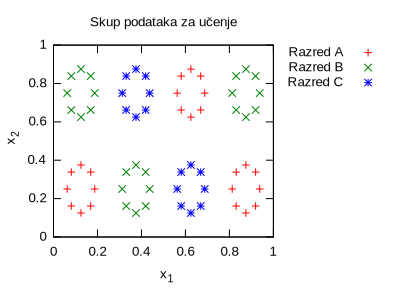
\includegraphics{img/task2-plot.pdf}
    \caption{Skup podataka za učenje
    \texttt{zad7-dataset.txt}}
    \label{z2-1}
\end{figure}

\pagebreak

\section*{Zadatak 3.}
Kada biste morali ručno odrediti vrijednosti svih parametara
upravo zadane neuronske mreže, na koje biste ih vrijednosti
postavili i zašto? Čime biste se vodili prilikom određivanja
parametara neurona skrivenog sloja a čime prilikom
određivanja parametara neurona izlaznog sloja? Nacrtajte tu
neuronsku mrežu i na njoj prikažite vrijednosti svih
parametara.

\section*{Rješenje:}
Razmatra se mreža čija je arhitektura $ 2 \times 8 \times 3 $
(skriveni sloj sastoji se od neurona tipa 1, a izlazni od
neurona tipa 2).

Neuroni prvog sloja trebali bi se specijalizirati za
računanje sličnosti ulaznog uzorka i nekog od 8 grupa
opisanih u prethodnom zadatku. Parametri jednog takvog
neurona $ w_1 $ i $ w_2 $ mogli bi se postaviti na centroid
odgovarajuće grupe uzoraka, dok bi se parametri $ s_1 $ i
$ s_2 $ mogli postaviti na neke vrijednosti manje od 0.1
($ s_1 $ bi trebao biti nešto manji od $ s_2 $ zbog izduženog
ovalnog oblika grupe).

Neuroni izlaznog sloja zaduženi su za klasifikaciju svake
grupe, odnosno odgovarajućeg neurona skrivenog sloja, u neki
od razreda. Prema tome, težina bi u tom sloju trebala imati
pozitivnu (veliku) vrijednost ukoliko povezuje neuron (grupu)
s pripadnim razredom, a negativnu (malu) ukoliko povezuje
neuron (grupu) s razredom kojemu taj neuron (grupa) ne
pripada. Slobodne težine bi u ovom slučaju trebalo postaviti
na 0 jer nisu potrebne.

Na slici \ref{z3-1} prikazano je moguće rješenje -- neuronska
mreža s vrijednostima parametara kako je iznad objašnjeno.
Ovakva mreža na ranije opisanom skupu podataka postiže
100\%-tnu ispravnost klasifikacije.

\begin{figure}
    \centering
    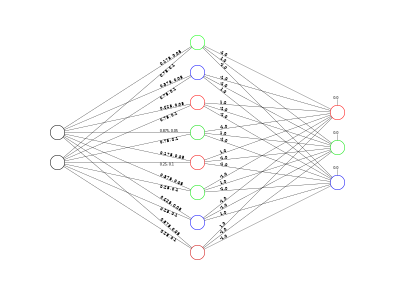
\includegraphics[width=\textwidth]
    {img/task3-neural-network.pdf}
    \caption{Neuronska mreža s ručno postavljenim parametrima}
    \label{z3-1}
\end{figure}

\pagebreak

\section*{Zadatak 4.}
Naučite optimalne parametre mreže arhitekture
$ 2 \times 8 \times 3 $. Nacrtajte novu sliku na kojoj se
vide svi ulazni uzorci s indikacijom razreda te uzorci koje
je GA naučio za svaki neuron tipa 1. Prokomentirajte gdje se
nalaze naučeni uzorci i je li to u skladu s očekivanjem.
Kakve je vrijednosti parametara $ s_i $ naučio GA? Jesu li
iste za $ x $ i $ y $ komponentu ili su različite?
Objasnite!\\
Nacrtajte novu sliku na kojoj se vide svi neuroni neuronske
mreže, pozicije koje su naučene u neuronima tipa 1 te
vrijednosti težina za neurone tipa 2. Uočavate li kakvu
pravilnost u tim težinama? Možete li je objasniti?

\section*{Rješenje:}
Na slici \ref{z4-1} prikazana je neuronska mreža s
parametrima koji su naučeni genetskim algoritmom. Genetski je
algoritam zaustavljen u 153892. iteraciji, nakon što je na
skupu za učenje postignuta srednja kvadratna pogreška iznosa
9.9593E-8.

Također, na slici \ref{z4-2} prikazan je skup podataka za
učenje s dodatno označenim naučenim uzorcima u neuronima tipa
1 prvog skrivenog sloja. Ti se naučeni uzorci nalaze blizu
središta eliptičnih grupa u skupu podataka, što je i u skladu
s očekivanjem. Vrijednosti parametara $ s_i $ također su u
skladu s očekivanjem -- radi se o vrijednostima čije su
apsolutne vrijednosti manje od 1. Za $ x $ komponentu su
nešto manje, kao što je bilo i očekivano s obzirom na
izduženost eliptičnih grupa u smjeru $ y $-osi.

Što se tiče težina neurona tipa 2, one su također očekivane.
Slobodne težine su malog iznosa, dok težine između skrivenog
i izlaznog sloja kodiraju odgovarajući razred. Doduše, iznosi
tih težina imaju poprilično veliku apsolutnu vrijednost što
bi se moglo protumačiti kao neki oblik prenaučenosti, ali je
genetski algoritam dovoljno rano (s dovoljno visokom
vrijednosti pogreške) zaustavljen pa je to donekle pod
kontrolom.

\begin{figure}
    \centering
    \includegraphics[width=\textwidth]
    {img/task4-neural-network.pdf}
    \caption{Neuronska mreža s parametrima naučenim
    genetskim algoritmom}
    \label{z4-1}
\end{figure}

\begin{figure}
    \centering
    \includegraphics{img/task4-plot.pdf}
    \caption{Skup podataka i naučeni uzorci u mreži
    $ 2 \times 8 \times 3 $}
    \label{z4-2}
\end{figure}

\pagebreak

\section*{Zadatak 5.}
Naučite optimalne parametre mreže arhitekture
$ 2 \times 8 \times 4 \times 3 $. Je li postupak učenja
trajao dulje ili kraće u odnosu na prethodnu arhitekturu?
Možete li objasniti zašto?\\
Pogledajte naučene parametre u neuronima tipa 1 za ovaj
slučaj. Možete li ih objasniti?

\section*{Rješenje:}
Postupak učenja traje kraće u odnosu na prethodnu
arhitekturu. Razlog tome je što je dodavanjem drugog
skrivenog sloja od 4 neurona, mreža dobila na ekspresivnosti
i nelinearnosti pa joj je lakše pronaći rješenje koje će
razdvojiti razrede (granice između razreda su slobodnije).

Naučeni uzorci u neuronima tipa 1 sada ne moraju biti u
središtima eliptičnih grupa jer se njihov loš razmještaj
može kompenzirati nelinarnim granicama u sljedećim slojevima.
Jedan njihov mogući naučeni razmještaj prikazan je na slici
\ref{z5-1}

\begin{figure}
    \centering
    \includegraphics{img/task5-plot.pdf}
    \caption{Skup podataka i naučeni uzorci u mreži
    $ 2 \times 8 \times 4 \times 3 $}
    \label{z5-1}
\end{figure}

\pagebreak

\section*{Zadatak 6.}
Možete li dobiti ispravnu klasifikaciju svih uzoraka u
arhitekturi koja ima $ N_1 < 8 $? Provjerite to na
arhitekturi $ 2 \times 6 \times 4 \times 3 $. Na kraju
(uspješnog ili neuspješnog) postupka učenja pogledajte za
najbolje rješenje parametre u neuronima tipa 1 za ovaj
slučaj. Što smo izgubili u odnosu na mrežu iz zadatka 4?

\section*{Rješenje:}
I u ovome se slučaju može dobiti ispravna klasifikacija svih
primjera. Naučeni parametri u neuronima tipa 1 vidljivi su na
slici \ref{z6-1}. Očito je da je dani skup podataka za učenje
moguće podijeliti linearnim granicama čak i s manje od 8
neurona tipa 1. Ipak, u odnosu na mrežu iz zadatka 4,
izgubljena je dobra interpretabilnost rješenja, odnosno
detekcija svih eliptičnih grupa, odnosno njihovih središta.

\begin{figure}
    \centering
    \includegraphics{img/task6-plot.pdf}
    \caption{Skup podataka i naučeni uzorci u mreži
    $ 2 \times 6 \times 4 \times 3 $}
    \label{z6-1}
\end{figure}

\end{document}